\documentclass{beamer} 

\mode<presentation>
{
  \usetheme{Berkeley}
  % or ...

  \setbeamercovered{transparent}
  % or whatever (possibly just delete it)
}

\usepackage{tikz}
\usepackage{graphicx}
\usepackage[english]{babel}
\usepackage{epstopdf}
\usepackage[utf8]{inputenc}
% or whatever

\usepackage{times}
\usepackage[T1]{fontenc}
% Or whatever. Note that the encoding and the font should match. If T1
% does not look nice, try deleting the line with the fontenc.


\title[Power and Multiple Hypothesis Testing] % (optional, use only with long paper titles)
{Power and Multiple Hypothesis Testing}

\subtitle
{}

\author[Christensen] % (optional, use only with lots of authors)
{Garret~Christensen\inst{1}}
% - Give the names in the same order as the appear in the paper.
% - Use the \inst{?} command only if the authors have different
%   affiliation.

\institute[Universities of Somewhere and Elsewhere] % (optional, but mostly needed)
{
  \inst{1}%
  UC Berkeley:\\
  Berkeley Initiative for Transparency in the Social Sciences\\
  Berkeley Institute for Data Science\\
  }
% - Use the \inst command only if there are several affiliations.
% - Keep it simple, no one is interested in your street address.

\date[BITSS2014] % (optional, should be abbreviation of conference name)
{IDB, March 2018\\
Slides available online at \url{http://www.github.com/BITSS/IDBMarch2018}}
% - Either use conference name or its abbreviation.
% - Not really informative to the audience, more for people (including
%   yourself) who are reading the slides online

\subject{Research Transparency}
% This is only inserted into the PDF information catalog. Can be left
% out. 

\pgfdeclareimage[height=2cm]{university-logo}{../Images/BITSSlogo.png}
\logo{\pgfuseimage{university-logo}}

% If you have a file called "university-logo-filename.xxx", where xxx
% is a graphic format that can be processed by latex or pdflatex,
% resp., then you can add a logo as follows:

% \pgfdeclareimage[height=0.5cm]{university-logo}{university-logo-filename}
% \logo{\pgfuseimage{university-logo}}



% Delete this, if you do not want the table of contents to pop up at
% the beginning of each subsection:
%\AtBeginSubsection[]
%{
%  \begin{frame}<beamer>{Outline}
%    \tableofcontents[currentsection,currentsubsection]
%  \end{frame}
%}


% If you wish to uncover everything in a step-wise fashion, uncomment
% the following command: 

\beamerdefaultoverlayspecification{<.->}


\begin{document}

\begin{frame}
  \titlepage
\end{frame}




% Structuring a talk is a difficult task and the following structure
% may not be suitable. Here are some rules that apply for this
% solution: 

% - Exactly two or three sections (other than the summary).
% - At *most* three subsections per section.
% - Talk about 30s to 2min per frame. So there should be between about
%   15 and 30 frames, all told.

% - A conference audience is likely to know very little of what you
%   are going to talk about. So *simplify*!
% - In a 20min talk, getting the main ideas across is hard
%   enough. Leave out details, even if it means being less precise than
%   you think necessary.
% - If you omit details that are vital to the proof/implementation,
%   just say so once. Everybody will be happy with that.
%%%%%%%%%%%%%%%%%%%%%%%%%%%%%%%%%%%%%%%%%%%%%%%%%%%%%%%%%%%%%%%%%%%%%%%
%%%%%%%%%%%%%%%%%%%%%%%%%%%%%%%%%%%%%%%%%%%%%%%%%%%%%%%%%%%%%%%%%%%%%
\begin{frame}{Outline}
  \tableofcontents
  % You might wish to add the option [pausesections]
\end{frame}

\section {Introduction}
{ % all template changes are local to this group.
    \setbeamertemplate{navigation symbols}{}
    \begin{frame}[plain]
        \begin{tikzpicture}[remember picture,overlay]
            \node[at=(current page.center)] {
                \href{https://www.bitss.org/}{\includegraphics[width=\paperwidth]{../Images/bitsslogo.png}}
            };
        \end{tikzpicture}
     \end{frame}
}

\begin{frame}{What is Statistical Power?}
The power of a statistical hypothesis test is the probability that the test correctly rejects the null hypothesis when it is false.
\vskip0.25in
That is, if there's a real effect, what's the likelihood you'll detect it? 80\% is the standard.
\end{frame}

\begin{frame}{What is Statistical Power?}
In terms of Type I (false positive) and Type II (false negative) errors: 
\begin{itemize}
\item Type I error rate is $\alpha$
\item Type II error rate is $\beta$
\item Power is $1-\beta$.
\end{itemize}
 \end{frame}

\begin{frame}{$Power=1-\beta$}
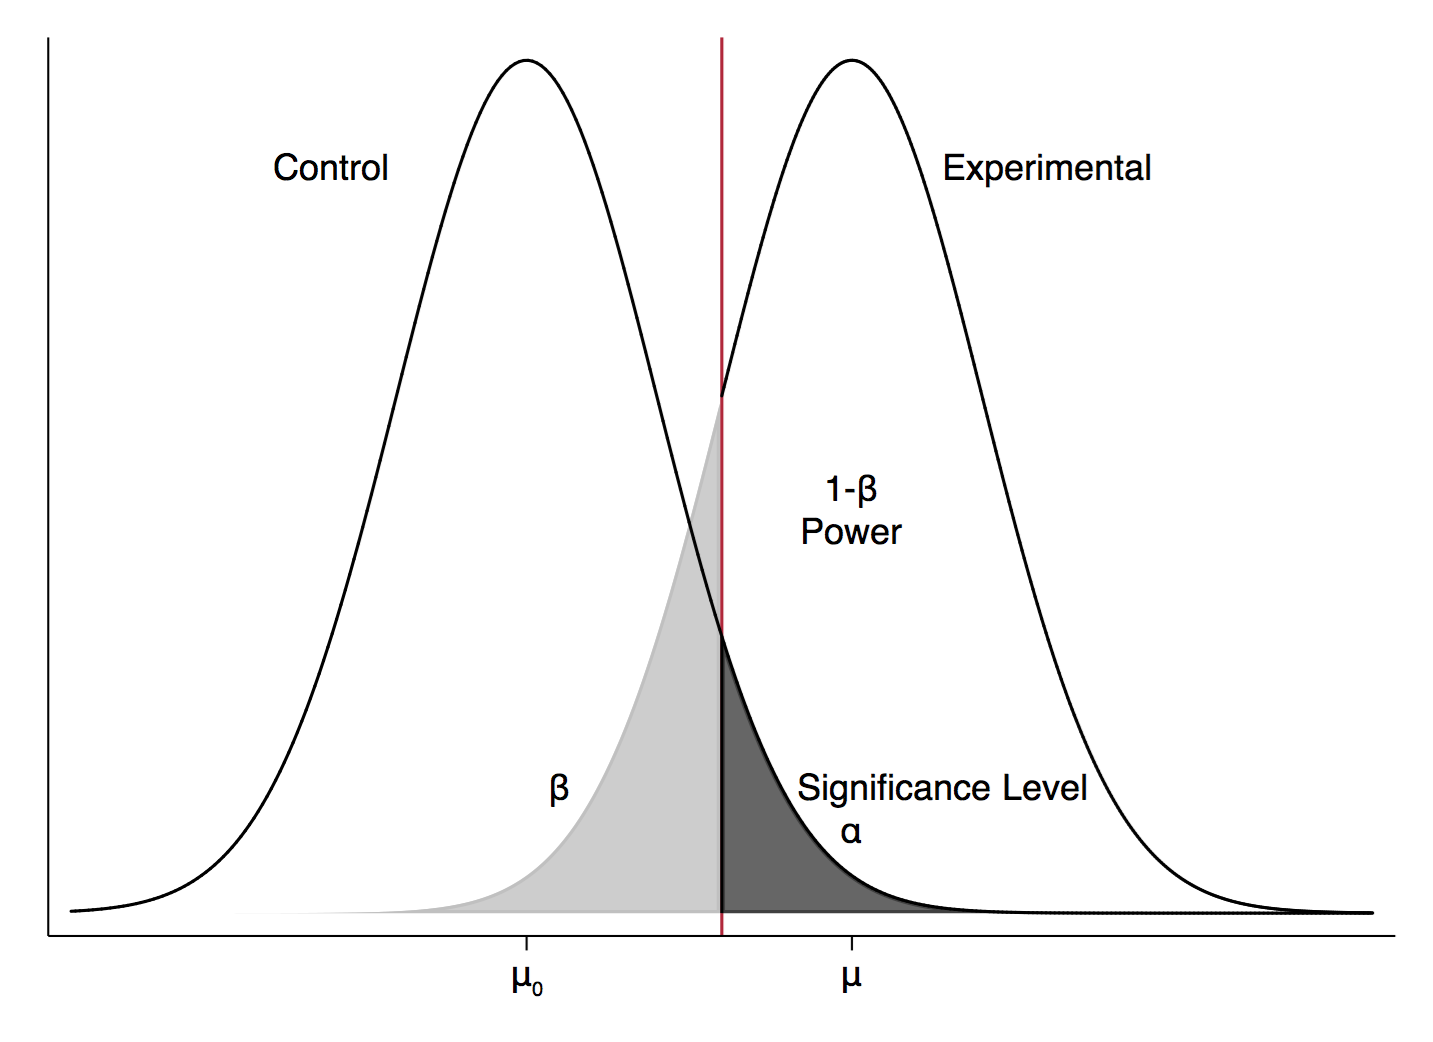
\includegraphics[height=3in]{../Images/powerfig1.png}
\end{frame}

\begin{frame}{Less noise, more power}
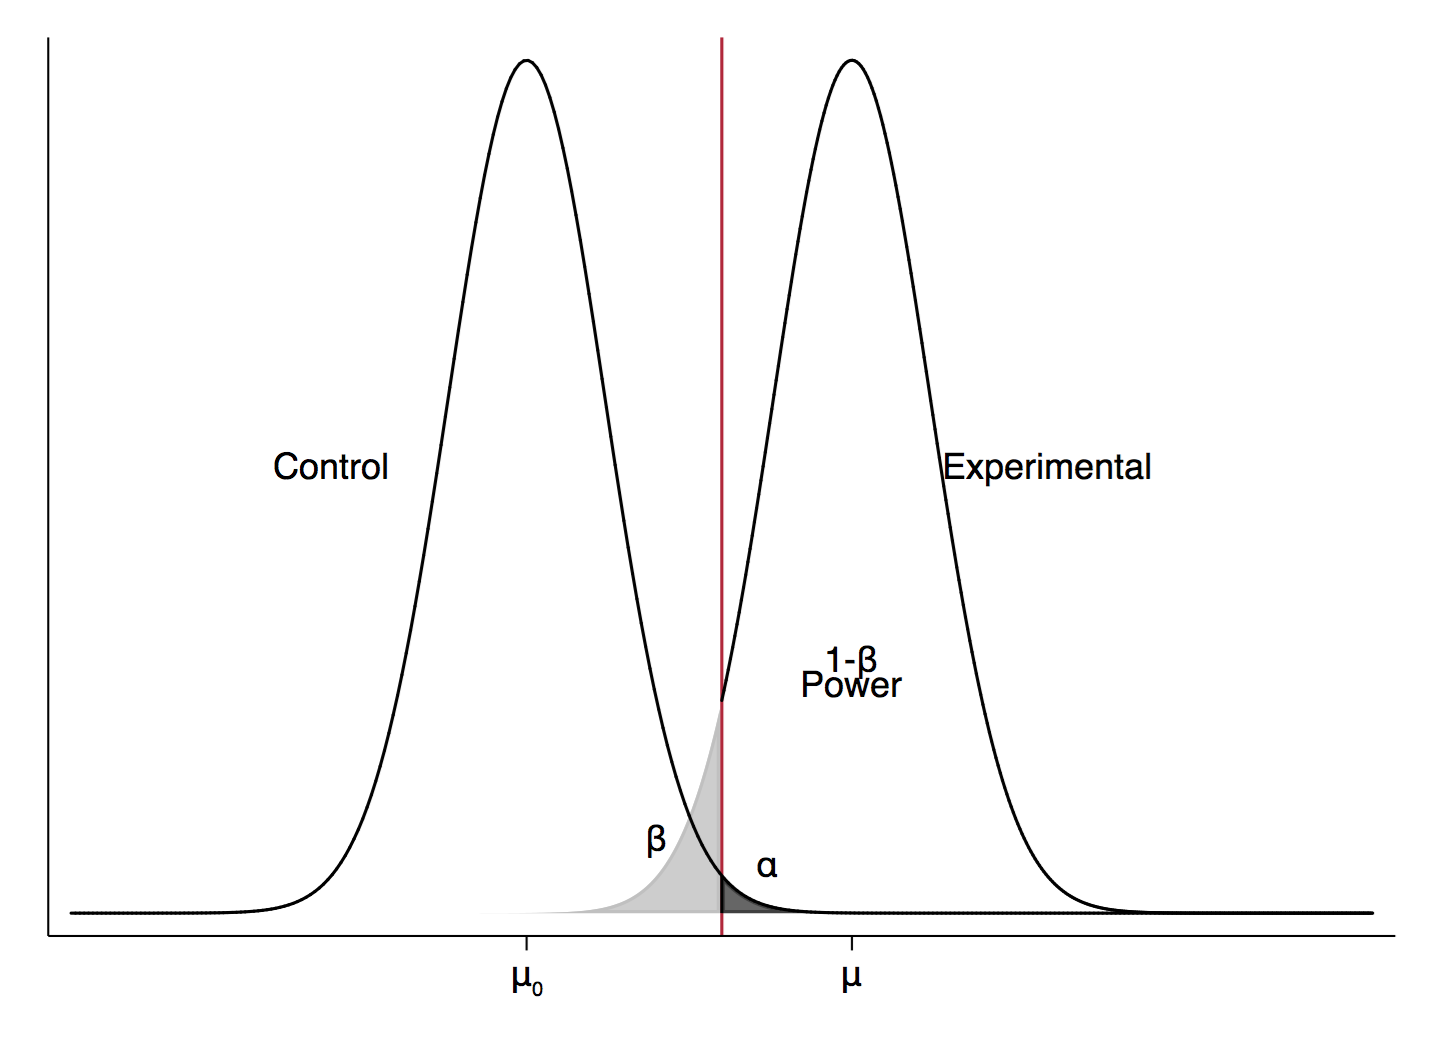
\includegraphics[height=3in]{../Images/powerfig2.png}
\end{frame}

\begin{frame}{Larger true effect, more power}
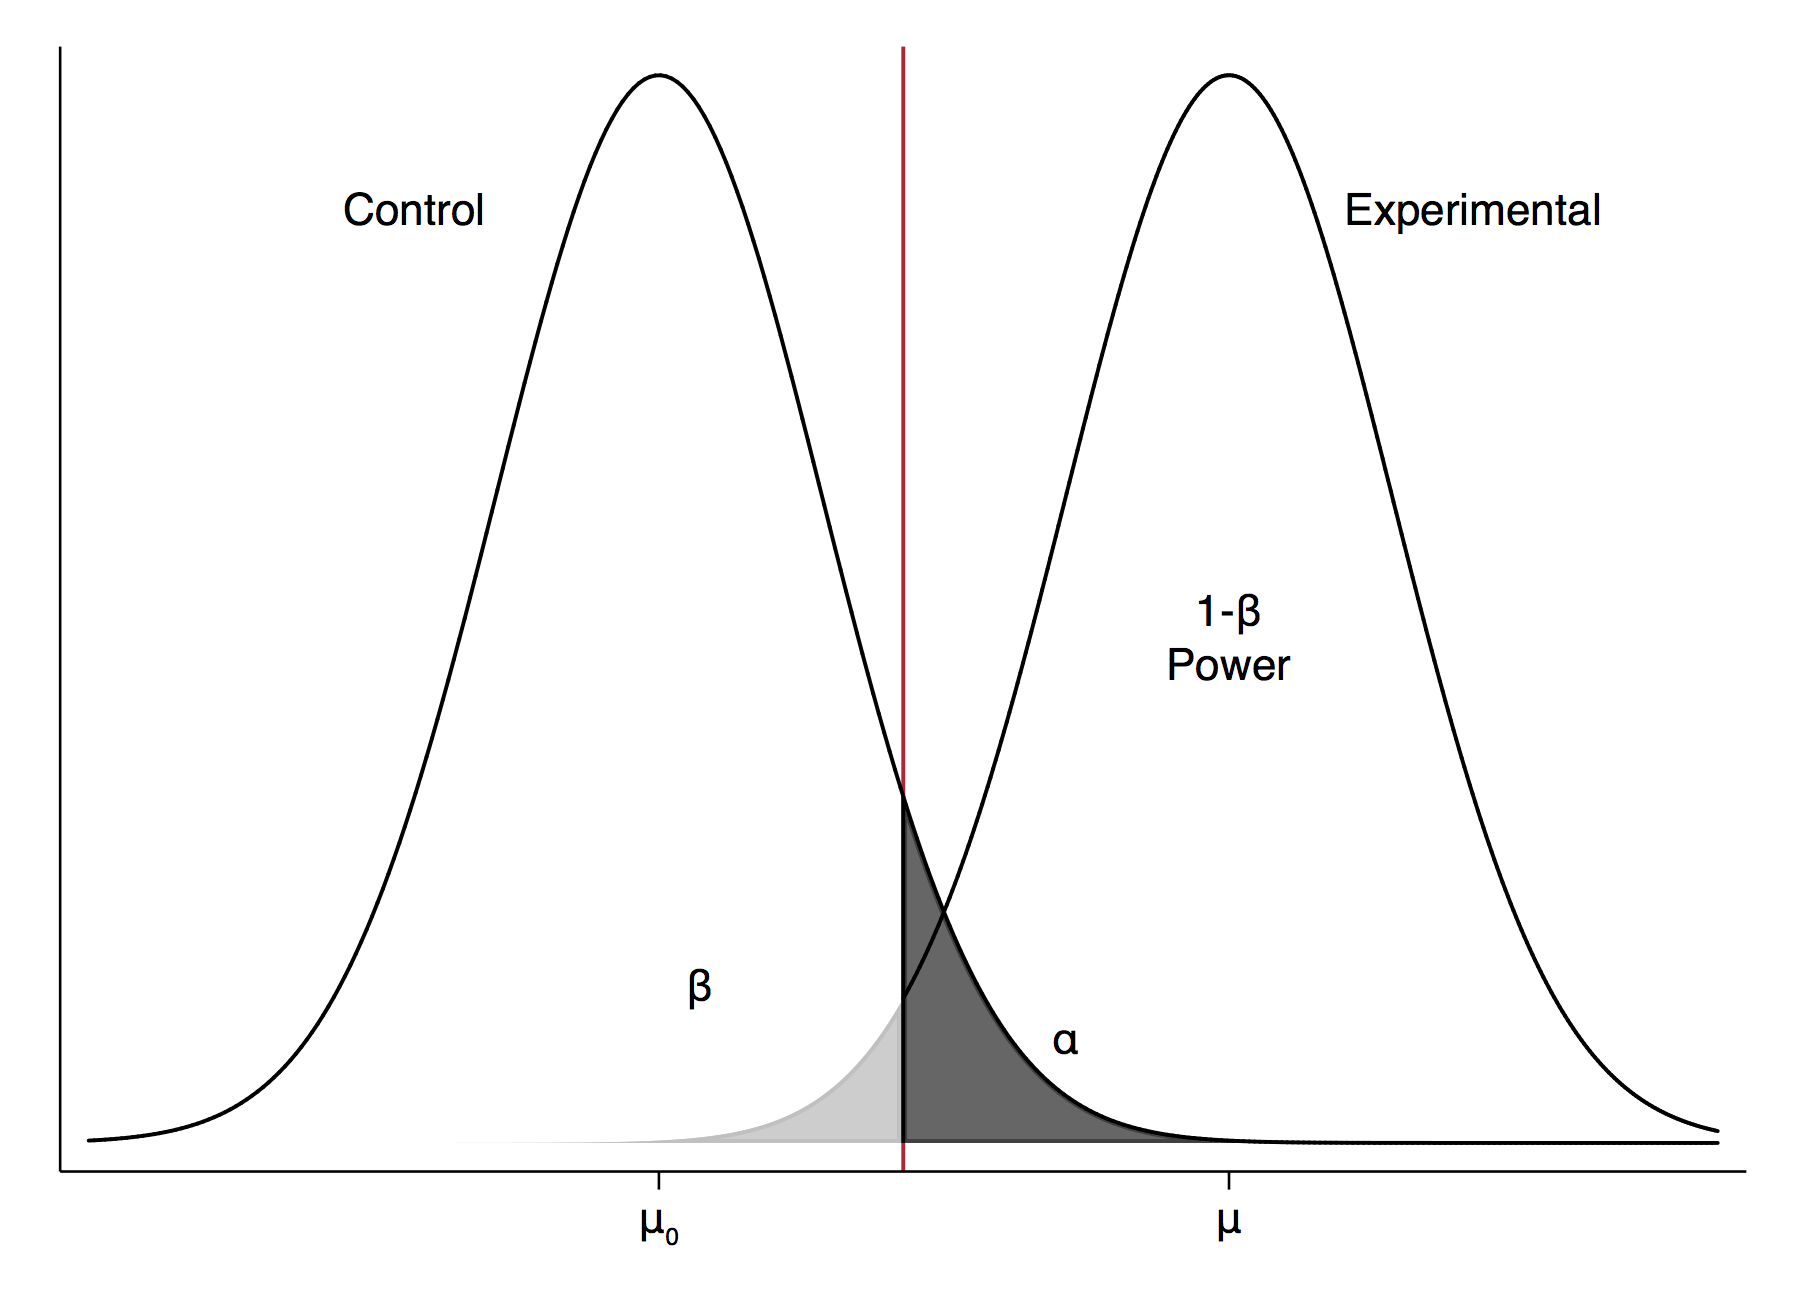
\includegraphics[height=3in]{../Images/powerfig3.png}
\end{frame}


\begin{frame}{Derivation}
\[Power = 1 - \beta = Pr(\overset{\overline{}}{Y} \geq \ \mu_{0} + z_{1 - \alpha}\sigma/\sqrt{}n|H_{1}:\ \mu > \mu_{0})\]

\[= 1 - Pr(\overset{\overline{}}{Y} < \ \mu_{0} + z_{1 - \alpha}\sigma/\sqrt{}n|H_{1})\]

\[= 1 - Pr(\frac{\overset{\overline{}}{Y} - \mu}{\frac{\sigma}{\sqrt{n}}} < \ \frac{\mu_{0} + \frac{z_{1 - \alpha}\sigma}{\sqrt{n}} - \mu}{\frac{\sigma}{\sqrt{n}}}|H_{1})\]

\[= 1 - Pr(\frac{\overset{\overline{}}{Y} - \mu}{\frac{\sigma}{\sqrt{n}}} < \ \frac{\mu_{0} - \mu}{\frac{\sigma}{\sqrt{n}}} + z_{1 - \alpha}|H_{1})\]

\[= 1 - \Phi(\ \frac{\mu_{0} - \mu}{\frac{\sigma}{\sqrt{n}}} + z_{1 - \alpha}|H_{1})\]

\[= \Phi(\ \frac{\mu_{0} - \mu}{\frac{\sigma}{\sqrt{n}}} - z_{1 - \alpha}|H_{1})\]
\end{frame}

\begin{frame}{Increasing Power}
\[= \Phi(\ \frac{\mu_{0} - \mu}{\frac{\sigma}{\sqrt{n}}} - z_{1 - \alpha}|H_{1})\]

Hopefully the equation makes clear that:
\begin{itemize}
\item larger $n$
\item lower $\sigma$
\item larger true effect size $(\mu_0-\mu)$
\item and a larger $\alpha$, though that's kind of cheating
\end{itemize}
 all increase power.
\end{frame}

\begin{frame}{Rearranging}
Rather than solving for power, you may want to solve for the minimum detectable effect (MDE). 

\[MDE = \left( t_{\beta} + t_{\alpha} \right)*\sqrt{\frac{1}{P(1 - P)}}\sqrt{\frac{\sigma^{2}}{n}}\]

Or, if you've got unlimited funds, pick the minimum biologically or practically meaningful effect, (or your estimate from previous literature of how big the effect will be) and solve for $n$.
\end{frame}

\begin{frame}{Design Effect}
We've so far assumed independent observations, which isn't the case if we cluster treatment. Multiply MDE by the Design Effect:

$$\sqrt{1+(n-1)\rho}$$

Where $n$ is households per sampling unit, and $\rho$ is the intracluster correlation--variance between clusters divided by sum of within and between.
\end{frame}

\begin{frame}{Complications}
Clusters not equal sized? Use the coefficient of variation, but it may not matter much. \href{https://doi.org/10.1093/ije/dyl129}{(Eldridge, Ashby, Kerry 2006)}
\vskip0.25in
You get the most power with equal proportions of treated/control. If treatment is very expensive, maximize power subject to your budget constraint. \href{http://www.sciencedirect.com/science/article/pii/S1573447107040612}{(Randomization Toolkit: Duflo, Glennerster, and Kremer 2007)}
\vskip0.25in
Panel with serial correlation? \href{https://static1.squarespace.com/static/558eff8ce4b023b6b855320a/t/59e932358dd041e0d712fff8/1508454965886/BPW\_Power\_Calculations\_2017\_10\_19.pdf}{(Burlig, Preonas, Woerman 2017)}
\vskip0.25in
Complicated? Simulate it. \href{https://doi.org/10.1186/1471-2288-11-94}{(Arnold et al. 2011)}
\end{frame}

\section{Problems in Econ}
\begin{frame}{Problem of Low Power}
So what happens if we have low power?
\begin{itemize}
\item
More false negatives (Type II error, just $\beta$).
\item
More false positives! More precisely, the likelihood that a reported effect represents a true finding decreases.
\end{itemize}
\end{frame}

\begin{frame}[label=Ioannidis]{Ioannidis 2005}
\href{http://journals.plos.org/plosmedicine/article?id=10.1371/journal.pmed.0020124}{``Why most published research findings are false'' (Ioannidis 2005)}, cited 5600 times.

\[PPV = Pr(True|T > t_{\alpha})\]


\[= \frac{(1 - \beta) \cdot R}{(1 - \beta)R + \alpha}\]

\begin{itemize}
\item
  R is ratio of true relationships to non-relationships tested in a literature.
\end{itemize}

\hyperlink{derive}{\beamerbutton{Derivation}}
\end{frame}

\begin{frame}{How Bad in Economics?}
\begin{quote} ``It's \textbf{bad}! It's REALLY \textbf{bad}.'' \\ \end{quote}
--Tom Stanley [Emphasis original]

\href{http://www.meta-analysis.cz/conference/Stanley_p.pdf}{\beamergotobutton{Source}}
\end{frame}

{ % all template changes are local to this group.
    \setbeamertemplate{navigation symbols}{}
    \begin{frame}[plain]q
        \begin{tikzpicture}[remember picture,overlay]
            \node[at=(current page.center)] {
                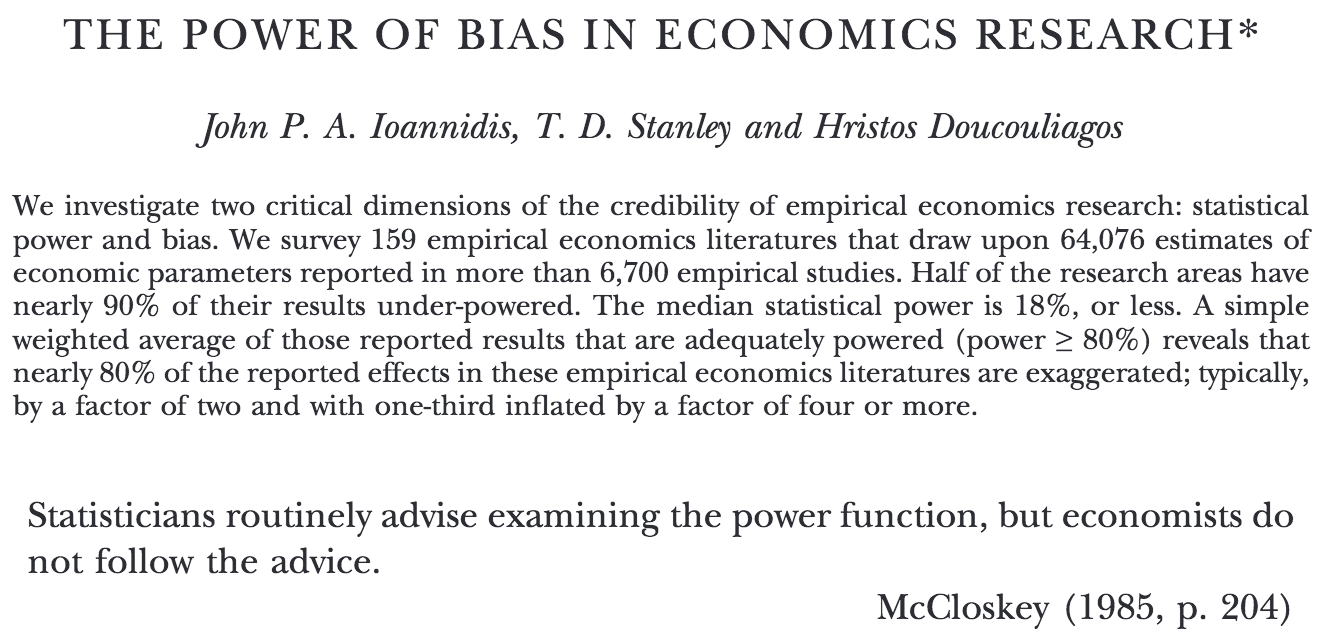
\includegraphics[width=\paperwidth]{../Images/Stanley2017.png}
            };
        \end{tikzpicture}
     \end{frame}
}

\begin{frame}{Ioannidis, Stanley, Doucouliagos 2017}
\begin{quote}If we adopt the conventional 5\% level of statistical significance and 80\% power
level, as well, then the `true effect' will need to be 2.8 standard errors from zero to
discriminate it from zero. The value of 2.8 is the sum of the usual 1.96 for a
significance level of 5\% and 0.84 that is the standard normal value that makes a 20/80\% split in its cumulative distribution. Hence, for a study to have adequate power, its
standard error needs to be smaller than the absolute value of the underlying effect
divided by 2.8. We make use of this relationship to survey adequate power in
economics.
\end{quote}
\end{frame}

\begin{frame}{Ioannidis, Stanley, Doucouliagos 2017}
But you still have to find the `true effect.' 

How? Meta-Analysis.
\begin{itemize}
\item simple weighted average of all estimates (`fixed effect')
\item same for top 10\% (smallest s.e.) estimates
\item single smallest s.e. estimate \href{https://www.sciencedirect.com/science/article/pii/S0022249613000278}{(Ioannidis 2013)}
\item meta-regression estimate (regress estimate on s.e., \href{http://onlinelibrary.wiley.com/doi/10.1111/j.1468-0084.2007.00487.x/full}{Stanley 2008)}
\end{itemize}
\end{frame}

\section{Multiple Testing}
\begin{frame}{Speaking of False Positives}
It's not just journals and researchers collectively creating publication bias, you can create the same problem all by yourself by testing multiple hypotheses and not adjusting for this. Especially if you only report the significant tests, but also if you report everything.
\vskip0.25in
P(false positive)$=\alpha$

P(no false positives)$=1-\alpha$

P(no false positives in m tests)$=(1-\alpha)^m$

P(at least one false positive in m tests)$=1-(1-\alpha)^m$
\end{frame}


{ % all template changes are local to this group.
    \setbeamertemplate{navigation symbols}{}
    \begin{frame}[plain]
        \begin{tikzpicture}[remember picture,overlay]
            \node[at=(current page.center)] {
                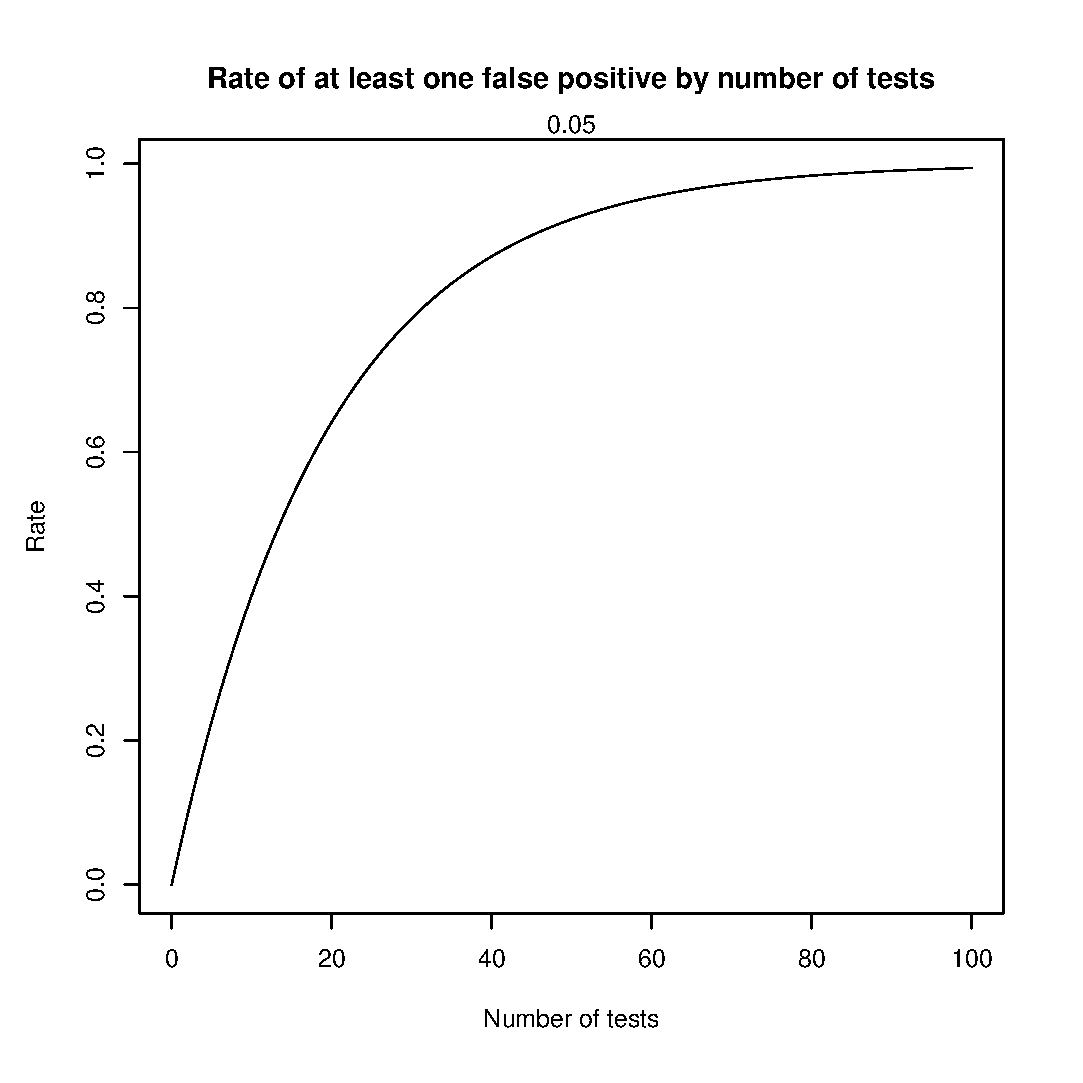
\includegraphics[height=\paperheight]{falsepositive.eps}
            };
        \end{tikzpicture}
     \end{frame}
}
\subsection{Index Tests}
\begin{frame}{Reduce Tests: Summary Index Tests}
Reduce number of tests conducted by grouping outcomes into indexes.
\begin{itemize}
\item Started with \href{http://www.jstor.org/stable/2531158}{O'Brien (1984)}
\item Economists know from \href{https://scholar.harvard.edu/lkatz/publications/experimental-analysis-neighborhood-effects}{MTO: Kling, Liebman, Katz (2007).}
\end{itemize}
How:
\begin{itemize}
\item Group outcomes into families
\item Align direction
\item Normalize and sum
\item Could also weight for more efficiency (unlikely to matter in practice)
\item Interpret as standard deviation unit
\end{itemize}
\end{frame}

\begin{frame}{Control the Type I Error Rate}
Primary methods:
\begin{itemize}
\item Family-wise error rate (FWER): the probability of at least one Type I error
\item False discovery rate (FDR): the expected proportion of Type I errors among rejected hypotheses
\end{itemize}
\end{frame}

\subsection{FWER Methods}
\begin{frame}{FWER Methods}
Bonferroni: divide your cutoff by the number of tests (or multiply p-value by number of tests, same thing)
\begin{itemize}
\item Not suggesting you do this
\item In fact, I am suggesting you \textit{not} do this 
\href{https://www.ncbi.nlm.nih.gov/pmc/articles/PMC1112991/}{(Pernerger 1998)}
\item It's just easy to understand
\end{itemize}
\end{frame}

\begin{frame}{Better FWER Methods}
\href{http://www.jstor.org/stable/2532216}{Westfall \& Young (1993)}: Free stepdown method
\begin{enumerate}
\item Sort by increasing \textit{p}-value
\item Simulate null data with resampling
\item Calculate simulated \textit{p}-values, $p^*_1, \ldots ,p^*_M$
\item Enforce original monotonicity $p^{**}_r=\min \{p^*_r \ldots p^*_M\}$ where $r$ is original rank
\item $L \geq 10,000$ repetitions, $S_r$ is number of times $p^{**}_r  < p_r$
\item $p_r^{fwer*}=S_r/L$
\item original monotonicity one more time: $p_r^{fwer}=\max \{p_1^{fwer*} \ldots p_r^{fwer*} \}$
\end{enumerate}
\end{frame}

\begin{frame}[label=FWERmain]{Free Stepdown}
\begin{itemize}
\item Dependence between outcomes preserved by resampling
\item Larger unadjusted \textit{p}'s correspond to larger adjusted \textit{p}'s
\end{itemize}
\hyperlink{FWERex}{\beamergotobutton{Example}}

\end{frame}

\subsection{FDR Methods}
\begin{frame}{FDR Methods}
Maybe one false positive isn't the end of the world, and you want more power. Control the expected proportion of false positives instead (FDR).
\vskip0.1in
Let $V=$ false rejections, $U=$ correct rejections, $t=$ total rejections.
\vskip0.1in
FWER is $P(V>0)$, FDR is $E[Q=V/t]$
\end{frame}

\begin{frame}{Benjamin Hochberg 1995}
\begin{enumerate}
\item Sort \textit{p}-values $1 \ldots M$
\item $q \in (0,1)$
\item Let $c$ be be largest $r$ for which $p_r<qr/M$
\item Reject all hypotheses $1 \ldots c$ to control FDR at $q$
\item That is, starting with $p_M$, check if $p_r<qr/M$. If true, reject it and all smaller $p$

\end{enumerate}
\end{frame}

\begin{frame}{Benjamini, Krieger, Yekutieli 2006}
Sharpen the procedure by estimating number of true null hypotheses
\begin{enumerate}
\item Apply BH  procedure at level $q'=q/(1+q)$. Let c be number of hypotheses rejected. Continue if $c\neq0$
\item Let $\hat{m}_0=M-c$
\item Apply BH at $q^*=q'M/\hat{m}_0$
\end{enumerate}
\vskip0.1in
Note: Procedures describe test for a given $q$, so test every value from $1, .999, .998 \ldots$ and find $q$ when hypothesis stops being rejected.
\end{frame}


\begin{frame}{Software}
\textbf{Stata}
\begin{itemize}
\item Michael Anderson
\begin{itemize}
\item Wonderfully written JASA paper \href{https://are.berkeley.edu/~mlanderson/pdf/Anderson\%202008a.pdf}{\beamergotobutton{Link}}
\item Stata for Benjamini \& Hochberg 1995 \href{http://are.berkeley.edu/~mlanderson/downloads/fdr_qvalues.do.zip}{\beamergotobutton{Link}}
\item Stata for Benjamini, Krieger, \& Yekuteli 2006 \href{http://are.berkeley.edu/~mlanderson/downloads/fdr\_sharpened\_qvalues.do.zip}{\beamergotobutton{Link}}
\end{itemize}
\item Roger Newson
\begin{itemize}
\item \texttt{ssc install qqplot} \href{http://www.stata-journal.com/sjpdf.html?articlenum=st0209}{\beamergotobutton{Stata Journal}}
\item \texttt{ssc install smileplot} \href{http://www.stata-journal.com/sjpdf.html?articlenum=st0035}{\beamergotobutton{Old Stata Journal}}
\end{itemize}
\end{itemize}
\textbf{R}
\begin{itemize}
\item p.adjust \href{https://www.rdocumentation.org/packages/stats/versions/3.4.3/topics/p.adjust}{\beamergotobutton{Link}}
\end{itemize}
\end{frame}

\begin{frame}{Active Area of Research}
List, Shaikh, Xu
\begin{itemize}
\item Useful in experimental economics:
\begin{itemize}
\item jointly identifying treatment effects for a set of outcomes
\item estimating heterogeneous treatment effects through subgroup analysis
\item conducting hypothesis testing for multiple treatment conditions
\end{itemize}
\item Builds on \href{https://projecteuclid.org/download/pdfview_1/euclid.aos/1262271625}{Romano, Wolf (2010)}
\item \href{http://www.nber.org/papers/w21875}{NBER WP}
\item \href{https://github.com/seidelj/mht}{Github (Stata, Matlab)}
\item \texttt{ssc install mhtexp}
\end{itemize}
\end{frame}

\section{Conclusion}
\begin{frame}{Conclusion}
\begin{enumerate}
\item Design studies with adequate power
\item Adjust for multiple tests
\begin{itemize}
\item Summary Indexes
\item FWER
\item FDR
\end{itemize}
\end{enumerate}

\end{frame}
%%%%%%%%%%%%%%%%%%%%%%%%%%%%%%%%%%%%%%%%%%%%%%%%%%%%%%%%%%%%%%%%%%%%%%%%%%

\begin{frame}
\begin{center}
Questions?
\vspace{1in}


\Huge{Thank you!}
\end{center}
\end{frame}


%%%%%%%%%%%%%%%%%%%%%%%%%%%%%%%%%%%%%%%%%%%%%%%%%%%%%%%%%%%%%%%%%%%%

\begin{frame}[label=derive]{Derivation of PPV I}
\[PPV = Pr(True|T > t_{\alpha})\]

Prior to the study, the quantities involved are as follows:

\begin{itemize}
\item
  Probability of a relationship being true: \(\frac{R}{R + 1}\)
\item
  Probability of a relationship being false:
  \(1 - \frac{R}{R + 1} = \frac{1}{R + 1}\)
\item
  Probability of finding a positive statistical association given that
  the relationship is false: \(\alpha\)
\item
  Probability of finding a positive statistical association given that
  the relationship is true (i.e., power): \(1 - \beta\)
\end{itemize}
\end{frame}

\begin{frame}[label=derive]{Derivation of PPV II}
Bayes' law says that \(Pr(A|B) = \frac{Pr(B|A)Pr(A)}{Pr(B)}\) , though
it is almost always the case that the denominator is more useful when
written out with the law of total probability, as follows:

\(Pr(A|B) = \frac{Pr(B|A)Pr(A)}{Pr(B|A)Pr(A) + Pr(B|\neg A)Pr(\neg A)}\).

By using Bayes' law, we know that:
\tiny{
\[Pr(True|T > t_{\alpha}) = \frac{Pr(T > t_{\alpha}|True) \cdot Pr(True)}{Pr(T > t_{\alpha}|True) \cdot Pr(True) + Pr(T > t_{\alpha}|False \cdot Pr\left( \text{False} \right))}\]}
\end{frame}

\begin{frame}[label=derive]{Derivation of PPV III}
Substituting, we find:

\[Pr(True|T > t_{\alpha}) = \frac{(1 - \beta)\frac{R}{R + 1}}{(1 - \beta)\frac{R}{R + 1} + \alpha \cdot \frac{1}{R + 1}}\]

\[Pr(True|T > t_{\alpha}) = \frac{\frac{(1 - \beta) \cdot R}{R + 1}}{\frac{(1 - \beta)R + \alpha}{R + 1}}\]

Simplifying:

\[Pr(True|T > t_{\alpha}) = \frac{(1 - \beta) \cdot R}{(1 - \beta)R + \alpha} = \frac{(1 - \beta)R}{R - \beta R + \alpha}\]

This is the same as the formula in Ioannidis (2005) and equation 1
above.
\hyperlink{Ioannidis}{\beamergotobutton{Back}}
\end{frame}

\begin{frame}[label=FWERex]{Free Stepdown Example}
Michael Anderson JASA 2008! \href{https://are.berkeley.edu/~mlanderson/pdf/Anderson\%202008a.pdf}{\beamergotobutton{Link}}
\vskip0.2in
``An example may aid interpretation of FWER-adjusted \textit{p}-values.
In this research, M = 9 summary indexes were tested for
each gender. Consider the smallest summary index \textit{p}-value of
the nine male summary indexes, which occurs for adult Early
Training males (Table 3). The unadjusted \textit{p}-value is approximately
.011. The corresponding adjusted \textit{p}-value, calculated
by the free step-down resampling method for the entire family
of male summary tests, is $p^{fwer} = .090$. Suppose that we simulate
the male data 100,000 times under the null hypothesis of no
treatment effect. 
\end{frame}

\begin{frame}{Free Stepdown Example II}
If we compute an entire set of nine summary
effect \textit{p}-values for each simulation, then the minimum \textit{p}-value
of that set will be less than or equal to the unadjusted \textit{p}-value of
.011 approximately 9\% of the time. Thus a minimum observed
\textit{p}-value of .011 is not unlikely under the null given the number
of tests conducted?a fact that helps explain why this particular
effect goes in the ``wrong'' (negative) direction. For unadjusted \textit{p}-values above the family's minimum \textit{p}-value, the number of
tests in the family effectively decreases, making the adjustment
less severe.''

\hyperlink{FWERmain}{\beamergotobutton{Back}}
\end{frame}



\end{document}


